\documentclass[12pt]{article}
\usepackage{sbc-template}
\usepackage{graphicx,url}
\usepackage[brazil]{babel}
\usepackage[utf8]{inputenc}
\usepackage{paralist}
\usepackage{graphicx}
\usepackage{subfig}
\usepackage{tabularx}
\usepackage{amsmath}
\usepackage{amssymb}
\usepackage{mathabx}

\sloppy

\title{Detecção de padrões de legendas em imagens de ritmo visual a partir
do detector de Harris}

\author{Guilherme Polo\inst{1}, Miguel Gaiowski\inst{1}}

\address{Instituto de Computação -- Universidade Estadual de Campinas
  (UNICAMP)\\
  Caixa Postal 6176 -- 13083-852 -- Campinas -- SP -- Brazil
  \email{\{ggpolo,miggaiowski\}@gmail.com}
}


\begin{document}
\maketitle

\begin{resumo}
  Vazio.
\end{resumo}


\section{Introdução}

\cite{harris}


\section{O detector de Harris}

A partir do detector de Moravec, definido em \cite{moravec}, ..

% XXX Pensando ...
%O detector de Harris \cite{harris} é classificado como um método
%baseado em intensidade \cite{detectors}.
% capaz de indicar pontos de borda
%e canto em uma imagem. Ele parte do detector de Moravec \cite{moravec}
%e descreve diversas melhorias sobre aquele 

Dada uma imagem $I$ e uma máscara $w$ ...

$w_{u,v} = \exp -\frac{u^2 + v^2}{2\sigma^2}$


% Produto de Hadamard: \circ
\begin{align*}
  X & = I \convolution [-1, 0, 1] \\
  Y & = I \convolution [-1, 0, 1]^\intercal \\
  A & = (X \circ X) \convolution w \\
  B & = (Y \circ Y) \convolution w \\
  C & = (X \circ Y) \convolution w
\end{align*}

Com $f \convolution h$ representando a convolução de $f$ com $h$ e
$M_1 \circ M_2$ sendo o produto de Hadamard que realiza a
multiplicação ponto a ponto entre as matrizes $M_1$ e $M_2$.

... explicação aqui .... Harris constroi a matriz R da forma seguinte:

\begin{align}
  Tr & = A + B \nonumber \\
  Det & = A \circ B - C \circ C \nonumber \\
  R & = Det - k (Tr \circ Tr) \label{REq}
\end{align}


... (visualização de uma matriz R na Figura \ref{figR}) ...

\begin{figure}[h]
  \centering
  \subfloat{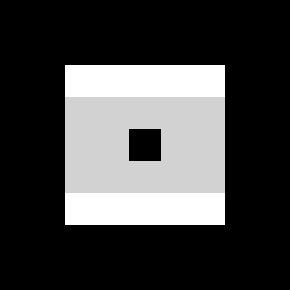
\includegraphics[height=4cm]{figs/sample_9_9.png}}\quad
  \subfloat{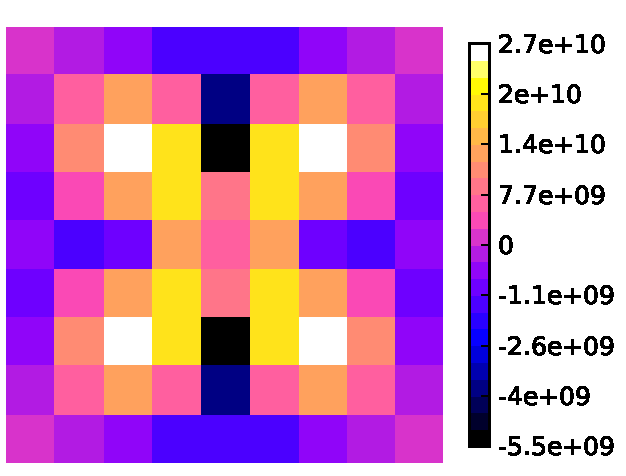
\includegraphics[height=4cm]{figs/sample_9_9_R}}
  \caption{Uma imagem 9x9 e sua respectiva matriz $R$ representada
    como um \textit{heatmap}\label{figR}}
\end{figure}


As Equações \ref{cornerEq} e \ref{edgeEq} definem, respectivamente, os
conjuntos de pontos de canto e de borda com base na matriz $R$. As
coordenadas $x$ e $y$ que não pertencem a $R$ são tomadas como não
definidas.

\begin{align}
  &\{(x, y) \mid \forall R[x,y] > 0 \bullet R[x,y] = \max(R[x-1:x+1,y-1:y+1)\} \label{cornerEq} \\
  &\{
    (x, y) \mid \forall R[x,y] < 0 \bullet \mbox{} \nonumber \\
  & \quad\quad\quad R[x,y] < \left\{
      \begin{array}{l l}
        min(R[x-1,y], R[x+1,y]) & \mbox{se} \,\, A[x,y] > B[x,y]\\
        min(R[x,y-1], R[x,y+1]) & \mbox{c.c.}\\
      \end{array}
    \right. \\ \label{edgeEq}
  &\} \nonumber
\end{align}

Na Equação \ref{cornerEq}, os pontos de canto que não são máximos ..

\section{Implementação}

Com a matriz $R$ (Equação \ref{REq}) construída e os pontos de canto
(Equação \ref{cornerEq}) e borda (Equação \ref{edgeEq}) definidos,
realizamos mais seis etapas. Na primeira, a partir de uma percentagem
do maior valor em $R$ descartamos os pontos de canto inferiores a este
valor. Na segunda, definimos um limiar inferior e superior -- também
com base numa porcentagem do maior valor absoluto de ponto de borda --
para os pontos de borda e classificamos cada borda de acordo com estes
limiares para, então, realizar a histerese. Estas duas primeiras
etapas são realizadas em cada banda da imagem e os resultados são
combinados numa única imagem. A imagem resultante até este passo é
formada pelas bordas e cantos escolhidas, com os cantos sendo
representados como um quadrado 3x3 centrado no ponto de canto real.

A partir deste ponto, são feitas tentativas para completar retângulos
quase fechados que possívelmente representam regiões de legenda nas
imagens de ritmo visual. Para cada ponto ainda não preenchido, é
verificado se ao menos um de seus vizinhos imediatos na horizontal
ou vertical foram preencidos. Caso algum deles tenham sido, este ponto
não preenchido é marcado para preenchimento no final deste processo.

Em seguida, o algoritmo \textit{flood fill} é aplicado para as
direções horizontais e verticais partindo do ponto $(0, 0)$. Nesta
implementação, este ponto, garantidamente, é inicialmente preto devido
a não consideração dos pontos em $R$, para construir as imagens até
este ponto, onde a máscara gaussiana escolhida não esta
inteiramente contida na imagem (considerando a convolução no domínio
espacial).

Na quinta etapa, os pontos que permanceram pretos são aqueles contidos
dentro de formas fechadas. Com isso, uma nova imagem é
criada para apresentar aqueles pontos pretos agora como brancos. Todos
os pontos brancos nesta imagem formam as possíveis regiões de
legenda. Como etapa final, é feita uma filtragem da mediana para
eliminar pequenas regiões que permaneceram devido a grande
heterogeneidade das imagens de ritmo visual.

\section{Avaliação}

Para realizar a avaliação, os parâmetros foram fixados para
todos os testes como: máscara guassiana 3x3 com $\sigma = 2$, limiar para
pontos de canto = $0.5 (\frac{max(R)}{100})$, limiares
$H = 2 (\frac{|min(R)|}{100})$ e $L = 0.01 (\frac{|min(R)|}{100})$ para
histerese e máscara 5x5 para filtragem da mediana.

De modo geral, o detector de Harris com os demais passos aplicados
foi capaz de encontrar regiões de legenda quando estas apresentavam um
contraste adequado na imagem como um todo. As Figuras
\ref{lowcontrast} e \ref{highcontrast} apresentam um resultado
considerado, por nós, ruim e outro bom.

\begin{figure}[h!]
  \centering
  \subfloat{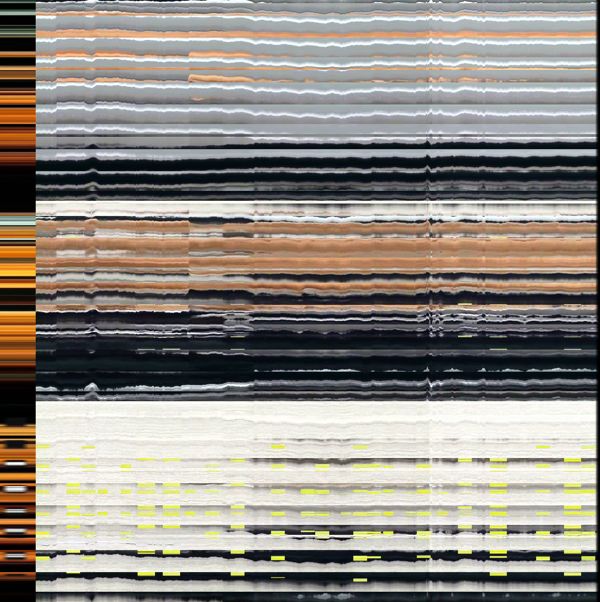
\includegraphics[width=0.45\linewidth]{figs/cats2.png}}\quad
  \subfloat{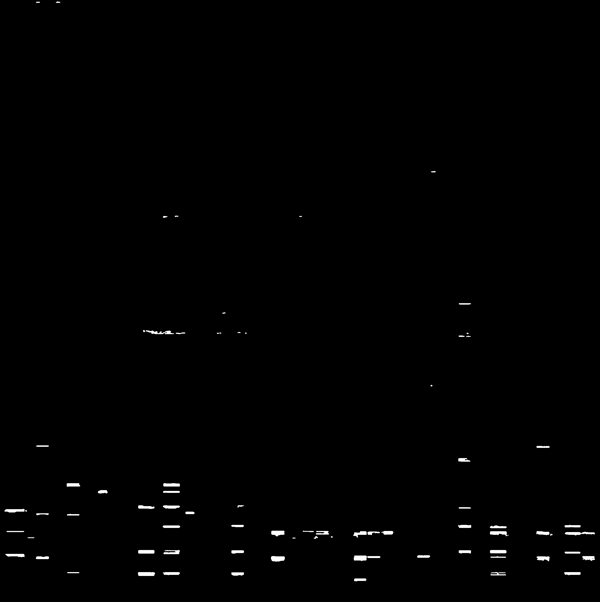
\includegraphics[width=0.45\linewidth]{figs/cats2_result.png}}
  \caption{Muitas regiões de legenda perdidas\label{lowcontrast}}
\end{figure}

\begin{figure}[h!]
  \centering
  \subfloat{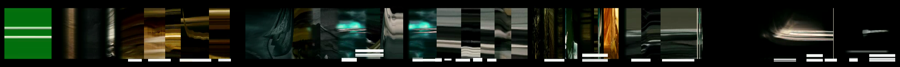
\includegraphics[width=\linewidth]{figs/harrypotter1.png}}\quad
  \subfloat{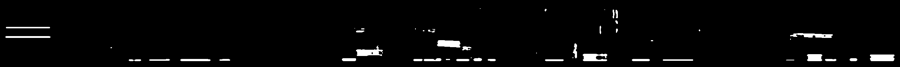
\includegraphics[width=\linewidth]{figs/harrypotter1_result.png}}
  \caption{Grande parte das regiões de legenda encontradas; alguns
    erros\label{highcontrast}}
\end{figure}

Na Figura \ref{lowcontrast}, acreditamos que cerca de seu um
terço superior não apresente legendas e nosso método detecta poucas
regiões nessa área. Entretanto, no segundo terço o método apresenta
falso-positivos em excesso. Na última parte desta imagem é onde grande
parte das legendas estão, mas a taxa de acerto foi baixa. Por outro
lado, a Figura \ref{highcontrast} apresenta o caso em que nosso método
tem bons resultados. Apesar de reportar incorretamente algumas partes
como sendo de legenda, todas as reais regiões de legenda
foram ao menos parcialmente indicadas.

...

\begin{figure}[h!]
  \centering
  \subfloat{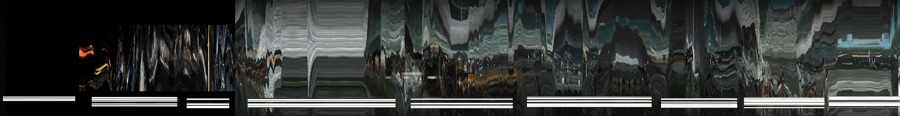
\includegraphics[width=\linewidth,height=1cm]{figs/t1_p1.png}}\quad
  \subfloat{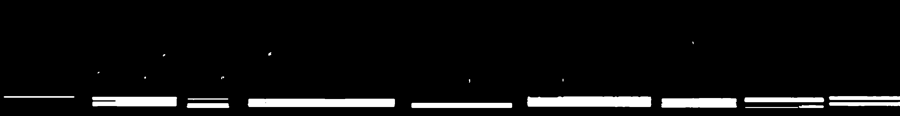
\includegraphics[width=\linewidth,height=1cm]{figs/t1r_p1.png}}\\
  \subfloat{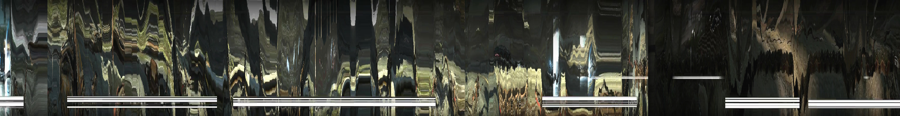
\includegraphics[width=\linewidth,height=1cm]{figs/t1_p2.png}}\quad
  \subfloat{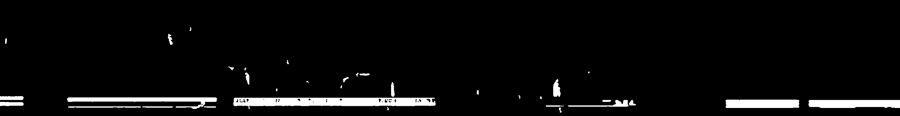
\includegraphics[width=\linewidth,height=1cm]{figs/t1r_p2.png}}\\
  \subfloat{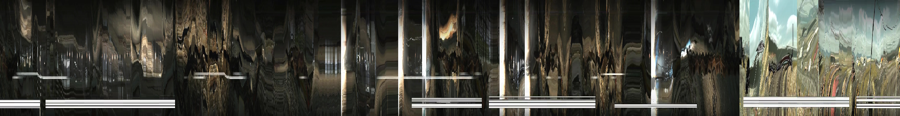
\includegraphics[width=\linewidth,height=1cm]{figs/t1_p3.png}}\quad
  \subfloat{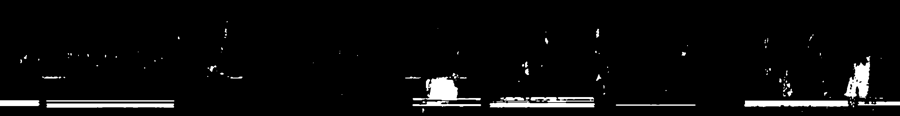
\includegraphics[width=\linewidth,height=1cm]{figs/t1r_p3.png}}\\
  \subfloat{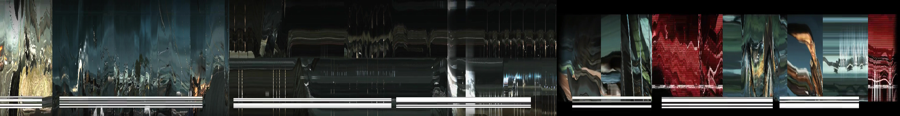
\includegraphics[width=\linewidth,height=1cm]{figs/t1_p4.png}}\quad
  \subfloat{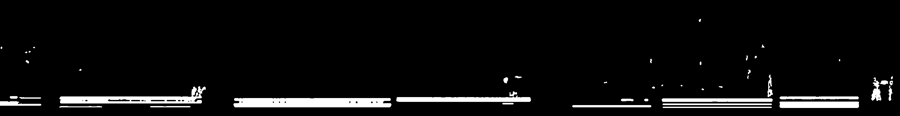
\includegraphics[width=\linewidth,height=1cm]{figs/t1r_p4.png}}\\
  \caption{...}
\end{figure}




\section{Conclusão}


\bibliographystyle{sbc}
\bibliography{biblio}

\end{document}
